%-----------------------------------------------------------------------
% Installation : Eclipse
% 
%-----------------------------------------------------------------------
\chapter{Installation des outils}

%-----------------------------------------------------------------------
\section{Eclipse}

L'environnement de développement utilisé est celui d'Eclipse\footnote{http://www.eclipse.org/}, éditeur très largement utilisé aujourd'hui pour les développements JAVA.

\medskip

\subsection{Téléchargement}
Vous pouvez télécharger Eclipse sur le 
\href{http://www.eclipse.org/downloads/}{site de téléchargement d'Eclipse}. A priori, toutes les versions destinées au développement Java devraient fonctionner. Néanmoins, seules les versions Helios(3.6), Indigo(3.7), Juno (4.2), Kepler (4.3) ont été testées dans le cadre de cette documentation. Le téléchargement de cette dernière version d'Eclipse pour les différentes plate-formes est directement accessible ici~:\\

\begin{center}
\begin{tabular}[!t]{lll}
Windows&
\href{http://www.eclipse.org/downloads/download.php?file=/technology/epp/downloads/release/kepler/R/eclipse-standard-kepler-R-win32.zip}{32bit}&
\href{http://www.eclipse.org/downloads/download.php?file=/technology/epp/downloads/release/kepler/R/eclipse-standard-kepler-R-win32-x86_64.zip}{64bit}\\
Mac OS X(Cocoa)&
\href{http://www.eclipse.org/downloads/download.php?file=/technology/epp/downloads/release/kepler/R/eclipse-standard-kepler-R-macosx-cocoa.tar.gz}{32bit}&
\href{http://www.eclipse.org/downloads/download.php?file=/technology/epp/downloads/release/kepler/R/eclipse-standard-kepler-R-macosx-cocoa-x86_64.tar.gz}{64bit}\\
Linux&
\href{http://www.eclipse.org/downloads/download.php?file=/technology/epp/downloads/release/kepler/R/eclipse-standard-kepler-R-linux-gtk.tar.gz}{32bit}&
\href{http://www.eclipse.org/downloads/download.php?file=/technology/epp/downloads/release/kepler/R/eclipse-standard-kepler-R-linux-gtk-x86_64.tar.gz}{64bit}\\
\end{tabular}
\end{center}

\medskip

\subsection{Installation}
Pour installer Eclipse, il suffit de décompresser le fichier téléchargé. 

\bigskip

\noindent
Lancer Eclipse :
\begin{itemize}
\item Sous windows cela crée un répertoire nommé "eclipse", exécuter le fichier eclipse.exe
\item Sous linux cela crée un répertoire nommé "/opt/eclipse", exécuter ./eclipse
\end{itemize}

\noindent
Lors du premier lancement, une boite de dialogue vous demandera de sélectionner le répertoire racine de vos projets Eclipse. Soit vous sélectionnez celui proposé, auquel cas il sera créé ou, vous pouvez en choisir un autre.

\newpage


%--------------------------------------------------------------------------
\subsection{Proxy}

Pour installer des mises à jour, de nouveaux plugins ou des extensions, il faut qu'Eclipse puisse accèder au net pour pouvoir les télécharger.  Si vous êtes derrière un proxy, il vous faut configurer Eclipse afin qu'il en tienne compte.

\bigskip

\begin{itemize}[leftmargin=* ,parsep=0cm,itemsep=0cm,topsep=0cm]

\item Pour ce faire, accéder au menu \emph{Window/Preferences/General/Network~Connection}. Vous pouvez alors séléctionner \emph{Manual} comme \emph{Active Provider} 

\begin{center}
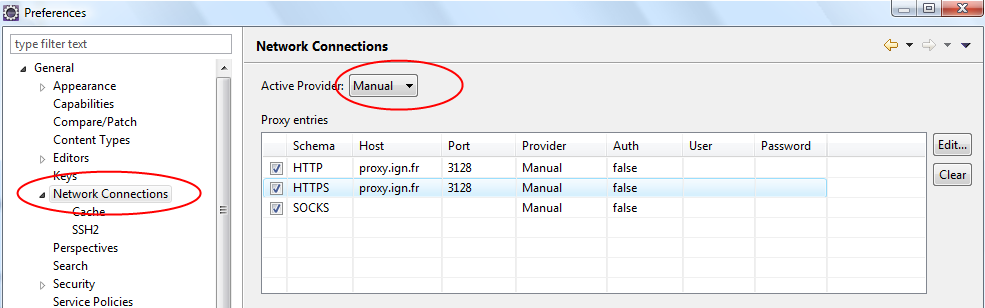
\includegraphics[width=0.8\linewidth]{proxy3}
\end{center}

\item Selectionner “HTTP” dans la liste des entrées et cliquer sur le bouton “Edit”

\begin{center}
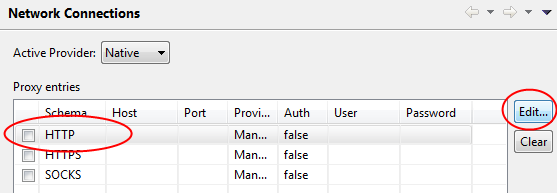
\includegraphics[width=0.5\linewidth]{proxy4}
\end{center}


\item Entrer les coordonnées de votre proxy. Pour l'IGN par exemple, il s'agit de \emph{proxy.ign.fr} avec le port \emph{3128}. Ne remplisser pas les champs d'authentification.

\begin{center}
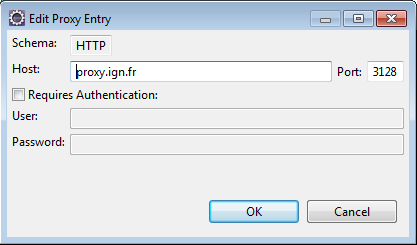
\includegraphics[width=0.4\linewidth]{proxy1}
\end{center}


\item Faire de même pour “HTTPS”

\begin{center}
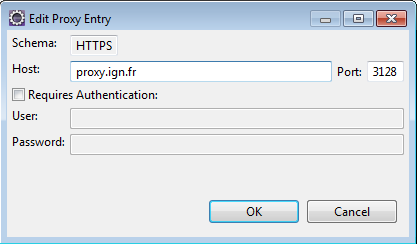
\includegraphics[width=0.4\linewidth]{proxy2}
\end{center}


\end{itemize}

%--------------------------------------------------------------------------

\subsection{Encodage}

Tous les modules de GeOxygène doivent être encodés en UTF-8. \\

\noindent
Pour ce faire, dans Eclipse :

Aller dans "Preferences $\Rightarrow$ Workspace $\Rightarrow$ Text file encoding $\Rightarrow$ Other"  et choisir UTF-8. 

\bigskip
\bigskip

%--------------------------------------------------------------------------


\noindent
Maintenant, Eclipse est prêt pour l'installation des plugins nécessaires à GeOxygene. Vous aurez besoin des plugins Maven (m2eclipse) et subversion (subclipse). Pour des questions de d\'ependance, il est pr\'ef\'erable de commencer par installer subclipse.

